\documentclass{ieeeaccess}
\usepackage{cite}
\usepackage{amsmath,amssymb,amsfonts}
\usepackage{algorithmic}
\usepackage{graphicx}
\usepackage{textcomp}

\usepackage{bm}
\makeatletter
\AtBeginDocument{\DeclareMathVersion{bold}
\SetSymbolFont{operators}{bold}{T1}{times}{b}{n}
\SetSymbolFont{NewLetters}{bold}{T1}{times}{b}{it}
\SetMathAlphabet{\mathrm}{bold}{T1}{times}{b}{n}
\SetMathAlphabet{\mathit}{bold}{T1}{times}{b}{it}
\SetMathAlphabet{\mathbf}{bold}{T1}{times}{b}{n}
\SetMathAlphabet{\mathtt}{bold}{OT1}{pcr}{b}{n}
\SetSymbolFont{symbols}{bold}{OMS}{cmsy}{b}{n}
\renewcommand\boldmath{\@nomath\boldmath\mathversion{bold}}}
\makeatother

\def\BibTeX{{\rm B\kern-.05em{\sc i\kern-.025em b}\kern-.08em
    T\kern-.1667em\lower.7ex\hbox{E}\kern-.125emX}}

%Your document starts from here ___________________________________________________
\begin{document}

\history{Date of publication xxxx 00, 0000, date of current version xxxx 00, 0000.}
\doi{10.1109/ACCESS.2017.DOI}

\title{Analysis of the Effectiveness of Super-Resolution Algorithms for Improving Computational Results: A Case Study on Two-Dimensional Diffusion Problems with Heterogeneous Coefficients}
\author{\uppercase{Ivan V. Konyukhov}\authorrefmark{1}
and \uppercase{Vladimir M. Konyukhov}\authorrefmark{2}}
\address[1]{Research Center of the Artificial Intelligence Institute, Innopolis University, Innopolis, 420500 Russia (e-mail: i.konyukhov@innopolis.ru)}
\address[2]{Research Center of the Artificial Intelligence Institute, Innopolis University, Innopolis, 420500 Russia (e-mail: v.konuhov.r@innopolis.ru)}
\tfootnote{The study was supported by the Ministry of Economic Development of the Russian Federation (agreement No. 139-10-2025-034 dd. 19.06.2025, IGK 000000C313925P4D0002).}

\markboth
{Konyukhov \headeretal: Analysis of the Effectiveness of Super-Resolution Algorithms...}
{Konyukhov \headeretal: Analysis of the Effectiveness of Super-Resolution Algorithms...}

\corresp{Corresponding author: Ivan V. Konyukhov (e-mail: i.konyukhov@innopolis.ru).}

\begin{abstract}
In this work, we explored the potential of using super-resolution techniques to reconstruct detailed concentration fields from their representations on coarse grids. We compared the performance of classical interpolation methods, such as bilinear and bicubic, with modern neural network-based approaches. It was demonstrated that intelligent algorithms, in particular those based on residual networks, demonstrated significant superiority in terms of reconstruction quality, as measured by the peak signal-to-noise ratio. These algorithms were also able to accurately reproduce the boundaries of complex geometric structures. Investigating the dependence of training quality on the balance of dataset,  the "hallucination" effect of the network was identified and analyzed. We also studied the computational efficiency of these methods, including training time and inference performance, while using central processing units, graphics processing units and neural processing units. It was demonstrated that the multi-scale deep super-resolution method showed the best results according to the criteria of reconstruction quality, training time and inference speed.
\end{abstract}

\begin{keywords}
diffusion, interpolation, machine learning, numerical methods,  super-resolution algorithms
\end{keywords}

\titlepgskip=-15pt

\maketitle

%============================================
\section{Introduction}
\label{sec:introduction}
%============================================
\PARstart{T}{he} solution to many problems related to modeling complex processes is obtained by using grid methods~\cite{Tikhonov_EMP}. The computational complexity of classical grid methods, such as finite difference and finite element methods, increases sharply with the number of spatial variables and required accuracy. This is especially true for two- and three-dimensional unsteady problems, where the demands on computational resources and solution speed become extremely high. Recently developed super-resolution algorithms have made it possible to significantly improve the computer modeling efficiency  of complex processes, see for example~\cite{Pathak_SR_CFD, Fukami_SR_CFD, Xie_SR_FF}. These methods allow us to reconstruct the calculated characteristics fields of the processes studied, which were obtained on coarse computational grids with small number of nodes, into the corresponding high-resolution fields by densifying the grids and increasing their size. By doing so, the computational load is shifted from computationally-extensive numerical modeling to the inference of a trained neural network and its execution on specialized hardware, such as graphics processors or neural processing units~\cite{Wang_SR_srv}.

Note that if the fields are constructed with a high degree of the details on grids with a greater number of nodes, then their representation on grids containing a smaller number of nodes (which obviously leads to a deterioration in their quality) can be achieved by solving a well-posed direct problem
%
%%%%%%%%%%%%%%%%%%%%%%%%%%%%%%
\begin{equation} \label{eq:degradation}
\mathrm{LR} = \mathrm{deg}(\mathrm{HR}),
\end{equation}
%%%%%%%%%%%%%%%%%%%%%%%%%%%%%%
%
where $\mathrm{deg}$ is a degradation function (e.g., due to blurring or noise addition);  $\mathrm{LR}$ and $\mathrm{HR}$ denote low-resolution and high-resolution fields, respectively. The inverse super-resolution problem 
$HR = {\deg ^{ - 1}}(LR)$ is the recovering a high-resolution field from its low-resolution version. Generally speaking, this is an ill-posed problem with no exact solution~\cite{Yang_DL_SR}.

Classical interpolation algorithms, such as linear and bicubic, are typical examples of super-resolution methods ~\cite{Getreur_LI}, which preceded the era of neural network algorithms based on deep learning. In particular, in one-dimensional case, linear interpolation allows the reconstruction of function values at intermediate nodes between two adjacent points on a coarse grid using the equation of a straight line. This ensures smoothness of the function up to the first-order derivative, but it can lead to blurring of piecewise continuous boundaries with the derivative discontinuities and loss of the fine details in the fields.

In turn, one-dimensional cubic interpolation uses a dependence constructed from four nodes of the coarse grid. Due to this fact, the reconstructed function is continuous with derivatives up to the second order and retains greater accuracy in intermediate nodes, although it takes more computational resources.

Similar problems arise when using bilinear and bicubic interpolation algorithms in two- and three-dimensional cases. However, despite their simplicity and high speed, these deterministic algorithms have fundamental limitations in their ability to recover high-frequency information that is lost during resolution reduction. This has led to the development of more advanced techniques based on neural networks that can learn complex structural patterns to reconstruct missing details ~\cite{Weiqin_SR}.

Currently, a large number of works are devoted to these problems. Without aiming to provide a detailed review and analysis of all of them, we mention some works as examples to demonstrate the variety of the approaches used for solving partial differential equations (PDEs). For instance, a thorough review of the findings on the use of super-resolution techniques can be found in ~\cite{Bin_SR_Review}.

The first neural network-based super-resolution algorithms  used convolutional neural networks (CNNs) ~\cite{Dong_SR}. CNNs are a type of deep learning algorithm that is designed to process data with a spatial structure, such as two-dimensional images and three-dimensional scenes. Their key distinction from ordinary fully connected networks lies in the use of convolutional layers, in which a small matrix (kernel) "slides" across the entire input image, computing scalar products and forming feature maps. By doing so, the network automatically extracts hierarchical features, starting from simple edges and textures in the initial layers of the network and progressing to more complex objects in deeper layers. Due to their properties such as translation invariance and efficient use of parameters, CNNs have become the basis for computer vision applications.

The Super-Resolution Convolutional Neural Network (SRCNN), introduced in ~\cite{Dong_SR}, enhances this approach. The SRCNN operates in three stages: (1) feature extraction, (2) non-linear mapping, and (3) final reconstruction. Unlike classical interpolation, SRCNN learns the convolutional kernel weights from a large dataset to minimize mean squared error (MSE) between the generated and ground truth high-resolution fields.

There are various strategies for using convolutional neural networks in "super-resolution" algorithms, see the review~\cite{Wang_SR_srv}. For example, some methods, such as the Very Deep Super Resolution (VDSR) algorithm ~\cite{Kim_VDSR}, use a preliminary increase in the number of  grid nodes (pre-upsampling) to construct a detailed solution. The Fast Super-Resolution Convolutional Neural Network (FSRCNN)  algorithm~\cite{Dong_FSRCNN} performs a post-increase the grid size (post-upsampling). The Laplacian Pyramid Super-Resolution Network (LapSRN)~\cite{Lai_LapSRCNN}, in turn,  uses a consequential increase in grid size (progressive upsampling) in the layers of the neural network, which is especially effective at higher values of the scaling factor.

%%%%%%%%%%%%%%%%%%%%%%%%%%%%%%%%%%%%%%%%%%%%%%%%%%%%%%%%%%%%%%%%%%%%%%%%%%%%%

A fundamental limitation in training deep convolutional neural networks is the "vanishing gradient problem", which is an exponential decrease in gradient magnitude as it propagates through the network, from output layers to input layers through successive layers. This is caused by the fact that gradients are calculated using the chain rule of differentiation, with multiple products of the derivatives, in error backpropagation process. This effect is most commonly seen with activation functions such as the sigmoid and hyperbolic tangent functions, which can lead to weights failing to update in earlier layers of the network, making deep learning inefficient or impossible, and limiting network's practical depth and ability to detect complex features
\cite{He_ResNet}.

Residual Networks (ResNets)~\cite{Zhang_ResSR} were specifically designed to solve the vanishing gradient problem in training very deep networks. Modern super-resolution algorithms, including Enhanced Deep Super-Resolution (EDSR)~\cite{Lim_EDSR} and Multi-scale Deep Super-Resolution (MDSR)~\cite{Gao_MDSR}, are built upon ResNet blocks. These models incorporate skip connections that allow the network to learn the residual, i.e. the difference, between a low-quality interpolated image and the target high-resolution image. The residual blocks primarily encode high-frequency components such as textures, edges and fine details thereby accelerating convergence and significantly improving reconstruction quality especially at high upscaling factors, e.g. $\times4$, $\times8$. Modified ResNet variants also show enhanced robustness to various artifacts and noise types, making them highly effective for solving computer vision problems \cite{He_ResNet}.

Such methods can also be effective in solving partial differential equations when the fields of physical characteristics are computed using numerical methods on coarse grids and then reconstructed using super-resolution algorithms on grids with a large number of nodes. This approach may significantly reduce the time required to solve the problem. However, it's necessary to note that if in standard image processing, perceptual quality is the primary metric, and minor structural hallucinations in natural images may be visually acceptable, then the application of super-resolution algorithms for solving differential equations can lead to the significant distortion of the real geometry and non-uniform structure of the solution region that invalidates the numerical results.

Note that new methods for solving PDEs have been developed recently by integrating physical constraints directly into super-resolution architectures. For example, \cite{Jiang_PCSR} proposes a physics-constrained framework for continuous space–time super-resolution in  the Rayleigh–Bénard convection problem, ensuring consistency with the governing flow equations. Similarly,  the paper  \cite{Kelshaw_PCSR} demonstrates the effectiveness of physics-informed CNNs in reconstructing sparse observations of dynamical systems with chaotic turbulent Kolmogorov flows. It is shown that this method outperforms classical interpolation methods in fine-scale reconstruction of turbulent structures, promising for experimental scenarios with limited measurement resolution. 

While physics-constrained methods provide physical consistency and data efficiency, purely data-driven models have certain advantages. In particular, they can learn implicit patterns directly from observations without requiring explicit physical constraints. They are also simpler to implement, train, and infer faster, because they avoid the expensive computation of PDEs residuals via automatic differentiation or finite difference approximations required by physics constrained methods. Therefore, our study focuses on evaluating the efficiency of established data driven architectures as a post processing tool for numerical PDEs solutions.

The goal of this research is to apply these algorithms to solving two-dimensional diffusion problems in regions with complex geometry and non-uniform diffusion coefficients. This work is an application-focused comparison study evaluating the performance of various neural network architectures, as well as identifying the conditions that lead to the "hallucination" effect during model training on imbalanced datasets, and providing practical guidelines for deploying super-resolution techniques on various computational platforms within scientific computing workflows. 

Note, that parabolic equations arise not only in modeling diffusion but also in heat conduction, migration of contaminants, multi-phase filtration  in non-uniform oil reservoirs, blood flow along the vessels with a porous thrombus on the walls, and other processes, see, for example \cite{Chekalin_2017,  Konyukhov_2020, Konyukhov_2022, Konyukhov_2023, Konyukhov_2025, Barenblat}.


%============================================
\section{Formulation of the Diffusion Problem and Its Numerical Solution}
%============================================

%============================================
\subsection{Problem Statement}
%============================================

Consider a homogeneous linear differential equation of parabolic type in a two-dimensional rectangular domain $\Omega = [0,T] \times [0,X] \times [0,Y]$ of a complex structure, where the unknown function $u(t,x,y)$ satisfies zero boundary conditions on all sides of the rectangle except for the top side and has a zero initial condition:
%
%%%%%%%%%%%%%%%%%%%%%%%%%%%%%%
\begin{equation}\label{eq:k15f}
    \frac{\partial u}{\partial t} = \frac{\partial}{\partial x}\left( D(x,y)\frac{\partial u}{\partial x} \right) + \frac{\partial}{\partial y}\left( D(x,y)\frac{\partial u}{\partial y} \right), 
\end{equation}
%%%%%%%%%%%%%%%%%%%%%%%%%%%%%%
$$
0 < x < X, \quad 0 < y < Y, \quad t > 0;
$$
%
\begin{equation}\label{eq:k16f}
    u(t,0,y) = 0; \quad  u(t,X,y) = 0; 
\end{equation}
\begin{equation}\label{eq:k16f_2}
    u(t,x,0) = 0; \quad u(t,x,Y) = U_Y;
\end{equation}
%
\begin{equation}\label{eq:k17f}
    u(0, x, y) = 0.
\end{equation}
%
For convenience in the subsequent discussion, let's assume that the process under consideration is the spreading of the concentration $u$ of a diffusing substance, and $D(x,y)$ is the diffusion coefficient.

%============================================
\subsection{Numerical Method}
%============================================

To test the neural network solution $\Psi$  generated by super-resolution algorithms, we will use the solution of the problem ~\eqref{eq:k15f}–\eqref{eq:k17f}, obtained by the finite difference method \cite{Samarskii, Süli}. 
Let us discretize the continuous domain  $\Omega$ using a uniform  grid of a finite  set of nodes $(t_k, x_i, y_j)$ and replace the governing equation~\eqref{eq:k15f} by an implicit finite-difference scheme with second-order approximation $O(h_t^2 + h_x ^ 2 + h_y^ 2)$:  
%
%%%%%%%%%%%%%%%%%%%%%%%%%%%%%%
\begin{equation}\label{eq:k18f}
    \frac{u_{i,j}^{k+1} - u_{i,j}^k}{h_t} = 
    \Lambda_x u_{i,j}^{(0.5)} + \Lambda_y u_{i,j}^{(0.5)}, 
    \end{equation}
%%%%%%%%%%%%%%%%%%%%%%%%%%%%%%
$$
          k = \overline{0,N_t-1}, 
    \quad i = \overline{1,N_x-1}, 
    \quad j = \overline{1,N_y-1};
$$
$$
\Lambda_x u_{i,j}^{(0.5)} = \frac{1}{h_x^2} ( D_{i - 1/2,j} \, u_{i - 1,j}^{(0.5)} - 
$$
$$
- (D_{i - 1/2,j} +  D_{i + 1/2,j}) \, u_{i,j}^{(0.5)} + D_{i + 1/2,j} \, u_{i + 1,j}^{(0.5)} ),
$$
$$
\Lambda_y u_{i,j}^{(0.5)} = \frac{1}{h_y^2} ( D_{i,j - 1/2} \, u_{i,j - 1}^{(0.5)} - 
$$
$$
- (D_{i,j - 1/2} + D_{i,j + 1/2}) \, u_{i,j}^{(0.5)} + D_{i,j + 1/2} \, u_{i,j + 1}^{(0.5)} ),
$$
%
where $t_k = k h_t$, $x_i = i h_x$, $y_j = j h_y$, $h_t = T/N_t$, 
$h_x = X/N_x$, $h_y = Y/N_y$, $k = \overline {0,{N_t}}$, $i = \overline {0,{N_x}} $, $j = \overline {0,{N_y}}$; $N_t$, $N_x$ and $N_y$ are the numbers of nodes along corresponding coordinate axes $t$, $x$ and $y$; 
$u_{i,j}^k = u({t_k},{x_i},{y_j})$;
$ u_{i,j}^{(0.5)} = (u_{i,j}^{k+1} + u_{i,j}^k)/2 $; 
${D_{i \pm 1/2,j}} = D\left( {{x_i} \pm {h_x}/2,{y_j}} \right)$;
${D_{i,j \pm 1/2}} = D\left( {{x_i},{y_j} \pm {h_y}/2} \right)$.

Following the longitudinal-transverse sweep method~\cite{Samarskii}, we introduce an intermediate time point $\bar{t} = t_{k+0.5}$ and subdivide the scheme~\eqref{eq:k18f} into two systems of algebraic equations:
%
%%%%%%%%%%%%%%%%%%%%%%%%%%%%%%
\begin{equation}\label{eq:k19f}
\frac{\bar{u}_{i,j} - u_{i,j}^k}{h_t/2} = \Lambda_x \bar{u}_{i,j} + \Lambda_y u_{i,j}^k,
\end{equation}
%%%%%%%%%%%%%%%%%%%%%%%%%%%%%%
%
\begin{equation}\label{eq:k20f}
\frac{u_{i,j}^{k+1} - \bar{u}_{i,j}}{h_t/2} = \Lambda_y u_{i,j}^{k+1} + \Lambda_x \bar{u}_{i,j}.
\end{equation}
%%%%%%%%%%%%%%%%%%%%%%%%%%%%%%

As shown in~\cite{Samarskii}, the longitudinal-transverse  scheme ~\eqref{eq:k19f} -– \eqref{eq:k20f} is equivalent to the original implicit scheme~\eqref{eq:k18f} and retains the second order  $O(h_t^2 + h_x^2 + h_y^2)$ of approximation.

The solution of systems proceeds in two steps. Firstly, the tri-diagonal system~\eqref{eq:k19f} is solved  with the one-dimensional sweep method along the $x$-direction, and as a result, the auxiliary grid function $\bar{u}_{i,j}$ is computed at the intermediate time point $\bar{t}$. Secondly, using the obtained $\bar{u}_{i,j}$, the desired solution $u_{i,j}^{k+1}$ is determined from the system~\eqref{eq:k20f} along the $y$-direction.

To maintain second-order accuracy in the first step, the boundary conditions at time $t_{k+0.5}$ for  
$i = 0$  and $i = N_x$ must be approximated using the following general relationship
$$
\bar{u}_{i,j} = \frac{1}{2} \left( u_{i,j}^{k+1} + u_{i,j}^k \right) - \frac{h_t}{4} \Lambda_y \left( u_{i,j}^{k+1} - u_{i,j}^k \right).
$$
However, in our case  the boundary conditions ~\eqref{eq:k16f} are homogeneous, then the correction term ${h_t}/4 \cdot {\Lambda _y}\left( {u_{i,j}^{k + 1} - u_{i,j}^k} \right)$ vanishes, yielding simply:
%
$$
\bar{u}_{0,j} = 0, \quad \bar{u}_{N_x,j} = 0, \quad j = \overline{0,N_y}.
$$
In the second step, approximation of the boundary conditions on $y = 0$ and $y = Y$ pose no difficulty, as they are prescribed on grid nodes $t_{k+1}$:
%
$$
u_{i,0}^{k+1} = 0, \quad u_{i,N_y}^{k+1} = U_Y, \quad i = \overline{0,N_x}.
$$

Note that since the longitudinal-transverse scheme  
~ \eqref{eq:k19f} -- \eqref{eq:k20f} is uniformly and unconditionally stable with respect to both the initial data and the right-hand sides ~\cite{Samarskii}, its convergence rate is $O(h_t^ 2 + h_x^2 + h_y^2)$.

%============================================
\subsection{Interpolation and Super-Resolution Algorithms}
%============================================

Usually, for example, in image processing, interpolation formulas, which only require the function values at the grid nodes, are often used.

\textbf{Bilinear interpolation.}

Let $u_{i,j}$ denote the values of the desired  discrete scalar function at grid nodes $(x_i, y_j)$,  $i = \overline{0,N_x}$, $j = \overline{0,N_y}$, and $\omega_ {i,j}$ is an arbitrary quadrilateral cell  defined by  vertices $(x_i, y_j)$, $(x_{i+1}, y_j)$, $(x_i, y_{j+1})$ and $(x_{i+1}, y_{j+1})$. The value of $u(x, y)$ at any  point $(x, y)$ inside $\omega_{i,j}$ can be calculated using the bilinear interpolation formula~\cite{Getreur_LI}:
%
%%%%%%%%%%%%%%%%%%%%%%%%%%%%%%
$$
u(x,y) = \frac{(y_{j + 1} - y)\big( u_{i,j}(x_{i + 1} - x) + u_{i + 1,j}(x - x_i) \big)}{(x_{i + 1} - x_i)(y_{j + 1} - y_j)} +
$$
%
\begin{equation}\label{eq:k23f}
+ \frac{(y - y_j)\big( u_{i,j + 1}(x_{i + 1} - x) + u_{i + 1,j + 1}(x - x_i) \big)}{(x_{i + 1} - x_i)(y_{j + 1} - y_j)}.
\end{equation}
%%%%%%%%%%%%%%%%%%%%%%%%%%%%%%
%
Formula~\eqref{eq:k23f} ensures the continuity of the function, but not its derivatives.

\textbf{Bicubic interpolation.}
First, we consider the construction of a one-dimensional cubic interpolation polynomial $u(x)$. In this case, the values of the functions $f_0 = u_{i-1}$, $f_1 = u_i$, $f_2 = u_{i+1}$ and $f_3 = u_{i+2}$ are defined not only at the nodes $x_i$ and $x_{i+1}$, but also at the neighboring points $x_{i-1}$ and $x_{i+2}$. The introduction of the normalized coordinate
$
\varsigma  = (x - x_i)/(x_{i+1} - x_i)
$
establishes a one-to-one correspondence between the points $x_{i-1}$, $x_i$, $x_{i+1}$, $x_{i+2}$ and $\varsigma_0 = -1$, $\varsigma_1 = 0$, $\varsigma_2 = 1$, $\varsigma_3 = 2$. The cubic interpolating polynomial on the interval $[-1, 2]$ can be written as ~\cite{Getreur_LI}
%
%%%%%%%%%%%%%%%%%%%%%%%%%%%%%%
$$
U(f_{0}, f_{1}, f_{2}, f_{3},\varsigma ) =
f_1 + \frac{1}{6}\Big[ (-2f_{0} - 3f_1 + 6f_2 - f_3)\,\varsigma +
$$
%
\begin{equation}\label{eq:k24f}
+ (3f_0 - 6f_{1} + 3f_2)\,\varsigma^2 
+ (-f_{0} + 3f_1 - 3f_2 + f_3)\,\varsigma^3 
\Big].
\end{equation}
%%%%%%%%%%%%%%%%%%%%%%%%%%%%%%
%
For any point $x\in [x_i, x_{i+1}]$, the interpolated value of the desired function $u(x)$ is obtained as
$$
u(x) = U\big(f_0, f_1, f_2, f_3, (x - x_i)/(x_{i+1} - x_i)\big).
$$

In the two-dimensional case, a bicubic polynomial is constructed similarly to formula ~\eqref{eq:k24f}, using the values of the grid function $u$ at the four nodes of the cell $\omega_{i,j}$ and at the twelve nodes of the neighboring cells $\omega_{i,j\pm 1}$, 
$\omega_{i \pm 1,j}$, and $\omega_{i \pm 1,j \pm 1}$. 
Let normalized coordinates be
$ \varsigma = (x - x_i)/(x_{i+1} - x_i)$ 
and $ \eta = (y - y_j)/(y_{j+1} - y_j)$. We denote the values of function at the nodes of these cells, as shown in Fig.~\ref{fig:Fig_1}. 
The values corresponding to the central cell $\omega_{i,j}$ are highlighted in bold.
%%%%%%%%%%%%%%%%%%%%%%%%%%%%%%
\Figure[ht!](topskip=0pt, botskip=0pt, midskip=0pt)[width=0.95\linewidth]{Konyu1.png}
{Numbering of grid function values in cells $\omega_{i,j}$, $\omega_{i,j \pm 1}$, $\omega_{i \pm 1,j}$, and $\omega_{i \pm 1,j \pm 1}$.
\label{fig:Fig_1}}
%%%%%%%%%%%%%%%%%%%%%%%%%%%%%%

A cubic polynomial of the variable $\varsigma$ is constructed for each row $m = -1, 0, 1, 2$ in a similar way to formula ~\eqref{eq:k24f}:
%
%%%%%%%%%%%%%%%%%%%%%%%%%%%%%%
\begin{equation}\label{eq:k25f}
R_m(\varsigma) = U(\phi_{m,0}, \phi_{m,1}, \phi_{m,2}, \phi_{m,3}, \varsigma), \quad m = \overline{0,3}.
\end{equation}
%%%%%%%%%%%%%%%%%%%%%%%%%%%%%%
%
Then, interpolation is done in the direction of $\eta$ using ~\eqref{eq:k25f}:
%
%%%%%%%%%%%%%%%%%%%%%%%%%%%%%%
\begin{equation}\label{eq:k26f}
\Phi (\varsigma ,\eta ) = U\big( R_0(\varsigma ), R_1(\varsigma ), R_2(\varsigma ), R_3(\varsigma ), \eta \big).
\end{equation}
%%%%%%%%%%%%%%%%%%%%%%%%%%%%%%
%
Thus, for any point $(x, y) \in \omega_{i,j}$,
$$
u(x,y)=\Phi ((x-x_i)/(x_{i+1}-x_i),
(y-y_j)/(y_{j+1}-y_j)).
$$

Note that bicubic interpolation~\eqref{eq:k25f}–\eqref{eq:k26f} ensures continuity of the first derivative and  provides more accurate results than bilinear interpolation, but requires more computational operations. Although bilinear interpolation is  not as accurate as bicubic interpolation, but it is easier to implement and faster to compute.


%============================================
\subsection{Super-Resolution Methods}
%============================================

We first consider super-resolution algorithms based on Convolutional Neural Networks (CNNs). Their  typical architecture is shown in Fig.~\ref{fig:Fig_2} and consists of the following sequential blocks.

\begin{enumerate}
 \item \textit{ Convolutional layers} for extracting features (properties, details, types, etc.) from input data elements.
 \item \textit {Subsampling (pooling) layers} for reducing the size of processed information while increasing the invariance of extracted features with respect to the location of objects in the input data.
\item \textit{Fully connected layers} performing the final function of classification or regression.
\end{enumerate}
%%%%%%%%%%%%%%%%%%%%%%%%%%%%%%
\Figure[ht!](topskip=0pt, botskip=0pt, midskip=0pt)[width=0.999\linewidth]{Konyu2.png}
{Architecture of a convolutional neural network.
\label{fig:Fig_2}}
%%%%%%%%%%%%%%%%%%%%%%%%%%%%%%

One of the most well-known CNN-based super-resolution algorithms is SRCNN (Super-Resolution Convolutional Neural Network), which is described in detail, for example, in~\cite{Dong_SR}.
In the preliminary stage of the SRCNN method, the low-resolution (LR) image is first enlarged to the desired size using a specified interpolation algorithm.
The resulting image is further denoted as IHR (Interpolated High-Resolution). The goal of the network is to transform the IHR into an SHR (Super-High-Resolution) image that closely approximates the original HR image. This process is realized in three stages.
\begin{enumerate}
    \item \textbf{Feature extraction}
At this stage, the first layer of the neural network takes an interpolated image as input. This image is then divided  into small patches, and convolutional filters are applied to generate high-level feature vectors for each selected area.
Rather than  using predefined features (for example, gradients), the  neural network learns on its own  which features are the most useful for subsequent reconstruction.
For this layer, you can set the size of the convolution core, which is usually 9x9; the number of filters,  for instance 64; and the activation function. Most commonly, the Rectified Linear Unit (ReLU) is used in neural networks to introduce non-linearity into the output of each neuron.

    \item \textbf{Non-linear mapping}.
The second layer is the most important layer in the neural network. It takes a feature vector from the first layer and and transforms it through a non-linear mapping into a feature vector representing a small patch of the IHR image.
This layer actually performs the main task of restoring high-frequency details that were  missing from in the original low-resolution image.
Similar to the previous layer, the size of the convolution core is usually set to 5×5, and the number of filters is 32. ReLU is also used as the activation function.

    \item \textbf{Final reconstruction}.
The third layer of the neural network takes an input vector of IHR image features from the second layer and processes them to create a final SHR image. This layer can be seen as the one that "puzzles together" the restored parts, ensuring the continuity and integrity of the final image. 
No activation function is typically used in this layer.
\end{enumerate}

The advantages of the SRCNN method include, firstly, its simplicity and fast training of a neural network.
Secondly, it significantly surpasses classical interpolation methods in terms of the quality of the resulting images. But also the method has some limitations.
%%%%%%%%%%%%%%%%%%%%%%%%%%%%
\begin{enumerate}
    \item  The neural network does not directly operate with the LR image, but requires its preliminary transformation into an IHR image. This process is computationally inefficient and may introduce noise into the image.
     \item One network is trained for a specific scaling factor  ($\times2$, $\times3$, $\times4$), 
     i.e., each scale requires its own model.
    \item Due to the small number of layers and their sizes, the network can only analyze small sections of the image at a time, which limits its ability to reconstruct the entire image.
\end{enumerate}
%%%%%%%%%%%%%%%%%%%%%%%%%%%%

Note that the SRCNN method formed the basis for all subsequent deep learning-based super-resolution models, such as FSRCNN, VDSR and LapSRN. These models eliminated  its limitations and improved image scaling results. Detailed description of the FSRCNN and VDSR methods can be found in  ~\cite{Dong_FSRCNN, Kim_VDSR}.
 For comparison, Table~\ref{tab:k1t} summarizes the key characteristics of SRCNN and VDSR only, as VDSR  actually generalizes capabilities found in FSRCNN and LapSRN.

%%%%%%%%%%%%%%%%%%%%%%%%%%%%%%
\begin{table}[ht]
\caption{Key characteristics of VDSR and SRCNN algorithms}
\setlength{\tabcolsep}{3pt}
\begin{tabular}{|p{35pt}|p{90pt}|p{95pt}|}
\hline
Parameter & VDSR & SRCNN \\
\hline
Network depth & 20 convolutional layers & 3 convolutional layers \\
\hline
Receptive field & Large ($41\times41$), it takes into account the global context & Small ($13\times13$), it is limited to the local context \\
\hline
Training speed & High, due to residual learning and gradient clipping & Slower than VDSR \\
\hline
Quality & Very high, especially at large scales & Good baseline, but inferior to VDSR \\
\hline
Scale support & Single model for multiple scales ($\times2$, $\times3$, $\times4$) & Separate model per scale \\
\hline
\end{tabular}
\label{tab:k1t}
\end{table}
%%%%%%%%%%%%%%%%%%%%%%%%%%%%%%

A common limitation of the above methods is the \textit{vanishing gradient problem}, which can hinder the deep training of  neural  networks.  As the network depth increases (e.g., to 50, 100 layers or more), the gradients that are transmitted back during training can become extremely small. This effectively stops the learning process. Modern approaches like EDSR and MDSR  are based on residual ResNet blocks ~\cite{Lim_EDSR, Gao_MDSR} and are devoid of this disadvantage. The ResNet architecture allows you to create models in hundreds and thousands of layers without performance degradation.

The main idea behind ResNet is to teach the \textit{residual function} $F(\chi)$ using residual blocks instead of a direct mapping $H(\chi)$, that is 
%%%%%%%%%%%%%%%%%%%%%%%%%%%%%%
$$
\mathcal{F}(\chi) = H(\chi) - \chi,
$$
%%%%%%%%%%%%%%%%%%%%%%%%%%%%%%
%
where $\chi$ is the block input. 
This is achieved by using skip connections, which bypass one or more layers. The block output is then $H(\chi)=\mathcal{F}(\chi)+\chi$. 
Such architecture of ResNet allows gradients to flow directly through the network during the error backpropagation, and makes it possible to effectively train networks with a depth of hundreds or even thousands of layers.

A typical residual block contains $3\times3$ convolutional layers. 
In this block, the batch normalization and the ReLU activation function are implemented. 
Bypass connections are organized between such blocks.
If the input and output sizes are different, the $1 \times 1$ convolutional layer   is used in the skip connection to equalize  these values.

A similar neural network architecture takes place in the implementation of the EDSR and MDSR methods.
In these models, the skip connections  enable the network to focus on identifying differences (i.e., textures, edges, fine details) between the interpolated LR image and the target HR image.  

This accelerates convergence and significantly improves reconstruction quality, especially at high upscaling factors ($\times4$, $\times8$). Comparative characteristics of the methods are given in Table~\ref{tab:k2t}.

%%%%%%%%%%%%%%%%%%%%%%%%%%%%%%
\begin{table}[ht]
\caption{Key characteristics of EDSR and MDSR algorithms}
\setlength{\tabcolsep}{3pt}
\begin{tabular}{|p{40pt}|p{85pt}|p{95pt}|}
\hline
Parameter & EDSR & MDSR \\
\hline
Primary purpose & Single-scale SR  (separate model per scale) & Multi-scale SR (single model for multiple scales) \\
\hline
Architecture & Deep residual network (32 blocks, 256 channels); batch normalization removed & Extended EDSR with scale-specific modules (two $5\times5$ residual blocks at input/output) \\
\hline
Number of parameters & Separate model of size $N$ for each scale $\times2$, $\times3$, $\times4$ & Single model of size $\approx N$ for all scales (3$\times$ more parameter-efficient) \\
\hline
Memory efficiency & High (no batch norm) & Very high (shared parameters across scales) \\
\hline
Quality & State-of-the-art for single-scale & Comparable to individual EDSR models per scale \\
\hline
Inference speed & Fast & Slower due to scale-specific modules \\
\hline
\end{tabular}
\label{tab:k2t}
\end{table}
%%%%%%%%%%%%%%%%%%%%%%%%%%%%%%

In the context of partial differential equations (PDEs), HR and SHR data represent physical fields that are calculated via numerical methods and super-resolution algorithms, respectively.
In the considered diffusion problem \eqref{eq:k15f}-\eqref{eq:k17f}, these data are the concentration fields $u(t,x,y)$ of the diffusing substance.
To solve this problem  and compare the results of our computational experiments, we use the currently most effective VDSR and MDSR methods.
Hereinafter, VDSR and MDSR are compared with the basic super-resolution algorithm (SRCNN), bilinear and bicubic interpolation methods.

%%%%%%%%%%%%%%%%%%%%%%%%%%%%%%
\subsection{Metrics for Evaluating the Quality of Reconstructed Fields}
%%%%%%%%%%%%%%%%%%%%%%%%%%%%%%

The quality of the reconstructed HR and SHR fields is evaluated with two standard metrics.
\begin{enumerate}
    \item \textbf{Mean Squared Error (MSE)} is
    %
    %%%%%%%%%%%%%%%%%%%%%%%%%%%%%%
    \begin{equation} \label{eq:k27f}
MSE = \frac{1}{{{N_x}{N_y}}}\sum\limits_i^{{N_x}} {\sum\limits_j^{{N_y}} {{{\left( {u_{i,j}^{HR} - u_{i,j}^{SHR}} \right)}^2}} }.
    \end{equation}
    %%%%%%%%%%%%%%%%%%%%%%%%%%%%%%
    %%%%%%%%%%%%%%%%%%%%%%%%%%%%%%  
    \item \textbf{The Peak Signal-to-Noise Ratio (PSNR)} is a widely applied  metric for  objectively assessing of the quality of reconstructed images, particularly in the tasks of image compression and super-resolution:
    %
    %%%%%%%%%%%%%%%%%%%%%%%%%%%%%%
    \begin{equation} \label{eq:k28f}
PSNR = 10{\log _{10}}\left( {{{{{\mathop {\max }\limits_{i,j} }^2}\left( {u_{i,j}^{HR}} \right)} \mathord{\left/
 {\vphantom {{{{\mathop {\max }\limits_{i,j} }^2}\left( {u_{i,j}^{HR}} \right)} {MSE}}} \right.
 \kern-\nulldelimiterspace} {MSE}}} \right).
    \end{equation}
    %%%%%%%%%%%%%%%%%%%%%%%%%%%%%%
\end{enumerate}

The correspondence between PSNR values and the quality of the reconstructed SHR image is summarized in Table~\ref{tab:k3t}, based on the empirical findings presented in~\cite{Wang}.
%%%%%%%%%%%%%%%%%%%%%%%%%%%%%%
\begin{table}[ht]
\caption{Interpretation of PSNR values}
%\label{table}
\setlength{\tabcolsep}{3pt}
\begin{tabular}{|p{39pt}|p{44pt}|p{145pt}|}
\hline
PSNR value & Image quality & Visual characteristics \\
\hline
$> 40$ dB & Excellent & Visually indistinguishable from the original; noise is virtually absent \\
30–40 dB & Good & High quality with minor distortions \\
20–30 dB & Fair & Noticeable but acceptable distortions \\
$< 20$ dB & Poor & Strong distortion and poor quality \\
\hline
\end{tabular}
\label{tab:k3t}
\end{table}
%%%%%%%%%%%%%%%%%%%%%%%%%%%%%%

It is important to note that, while PSNR and MSE provide standard measures of structural and numerical fidelity between reconstructed and reference fields, they do not inherently enforce physical conservation laws or guarantee satisfaction of the underlying PDE residuals. Consequently, they should be interpreted primarily as indicators of spatial reconstruction accuracy rather than strict physical correctness.



%============================================
\subsection{Neural Network Training Methodology}
%============================================

To prepare datasets for training various super-resolution neural models, we generate paired LR and HR samples by solving the diffusion problem on the grids with small and large numbers of nodes under diverse initial data. 
Let us illustrate this process on the example of preparing spatial maps of the diffusion coefficient $D(x, y)$, which are used to compute concentration fields $u(t,x,y)$.

Since the accuracy of difference schemes on the LR-grids is lower than on HR-grids, it is advisable to use not just a subdiscretization approach for model training when the concentration values at the nodes of the LR-grid are taken from the HR-solution. Instead, it should be done by comparing the LR and HR numerical solutions. 
These paired concentration maps, corresponding to the same time instants $t$ but generated for different spatial distributions of $D(x,y)$ (which play the role of textures), constitute the training dataset.
 
To ensure a fair comparison, all algorithms are trained on the same fixed dataset consisting of samples with varying geometric structures (or textures).

We consider the following variants of the model distribution $D(x, y)$  within the heterogeneity region $\omega$ consisting of  both straight and curved boundaries  in the diffusion problem~\eqref{eq:k15f}–\eqref{eq:k17f}.

\begin{enumerate}
    \item $D(x, y) = D_0 = \mathrm{const}$ for $(x, y) \in \Omega$.  
 This variant allows the neural network model to be trained for creating a solution in the homogeneous diffusion domain $\Omega$ without any heterogeneous inclusions.
    
    \item The diffusion coefficient is piecewise constant:
    %
    %%%%%%%%%%%%%%%%%%%%%%%%%%%%%%
    $$
    D(x, y) = 
        \begin{cases}
            D_0, & (x, y) \in \Omega \setminus \omega, \\
            D_1, & (x, y) \in \omega,
        \end{cases}
    $$
    %%%%%%%%%%%%%%%%%%%%%%%%%%%%%%
    where $D_1 \ne D_0$;  $\omega \subset \Omega$ is a geometric inclusion of varying shape (e.g., circle, triangle, square).  
    These configurations are designed to train the network for accurate reconstructing sharp boundaries of heterogeneous domains of different geometries (see Fig.~\ref{fig:Fig_3}(a)).
 
    \item The region $\omega$ has a different geometric shape and a spatial layered heterogeneous structure with respect to the diffusion coefficient:
    %
    %%%%%%%%%%%%%%%%%%%%%%%%%%%%%%
    $$
    D(x,y) = 
    \begin{cases}
        D_0, & (x,y) \in \Omega \setminus \omega, \\
        D_1(x,y), & (x,y) \in \omega,
    \end{cases}
    $$
    %%%%%%%%%%%%%%%%%%%%%%%%%%%%%%
      where the level lines of the function $D_1(x,y)$ repeat   the shape of $\partial\omega$. The function $D_1(x,y)$ may either increase (Fig.~\ref{fig:Fig_3}(b)) or decrease (Fig.~\ref{fig:Fig_3}(c)) from the center of region $\omega$ towards its boundary. In the figures, darker-to-lighter color transitions correspond to increasing values of $D_1(x,y)$.
  
\end{enumerate}

%%%%%%%%%%%%%%%%%%%%%%%%%%%%%%
\Figure[ht!](topskip=0pt, botskip=0pt, midskip=0pt)[width=0.999\linewidth]{Konyu3.png}
{Examples of heterogeneity regions $\omega$ with different structures: (a) case~2; (b) and (c) case~3.
\label{fig:Fig_3}}
%%%%%%%%%%%%%%%%%%%%%%%%%%%%%%

Since $D(x,y)$ is a table function defined in $\Omega$ and $\omega\setminus\Omega$, the resulting concentration field $u(t,x,y)$ inherits the structural features of $D(x,y)$. This is illustrated in Fig. \ref{fig:Fig_4}.

%%%%%%%%%%%%%%%%%%%%%%%%%%%%%%
\Figure[ht!](topskip=0pt, botskip=0pt, midskip=0pt)[width=0.999\linewidth]{Konyu4.png}
{Concentration fields $u(x,y)$ corresponding to circular and triangular inclusions $\omega$ which are shown in Fig.~\ref{fig:Fig_3}(a) and~\ref{fig:Fig_3}(b), respectively.
\label{fig:Fig_4}}
%%%%%%%%%%%%%%%%%%%%%%%%%%%%%%

Generating LR–HR pairs requires repeatedly solving the diffusion problem, which can be computationally intensive.  In addition, finite-difference implementations in interpreted languages such as Python often involve deeply nested loops, significantly limiting performance.
To accelerate computations, the \textit{Just-In-Time} (JIT) compiler library \textit{Numba} can be used ~\cite{Lam}. It translates the Python modules and NumPy-based mathematical expressions into optimized machine code at runtime, yielding speedups of \textasciitilde100 -- 10000 times. 

Due to the JIT compilation and parallelization features, \textit{Numba} significantly reduces the dataset preparation time from hours to minutes, allowing for training on large and various datasets. For instance, solving the diffusion problem on a grid of $16 \times 16 \times 256$ nodes takes only 0.007 seconds using \textit{Numba}, as opposed to 10 seconds without it, resulting in a speedup of more than 1300 times.

As shown in~\cite{Weiqin_SR}, the loss function $L(\vec{\theta})$ for training of the super-resolution models on  dataset $\vec{\theta}$ is usually calculated as the mean squared error between HR- and SHR-images, which in our case are concentration fields ${u_{i,j}^{HR}}$ and ${u_{i,j}^{{SHR}}}$, respectively. Then 
$
 \mathcal{L} (\vec{\theta}) = MSE(\vec{\theta}),
$
%%%%%%%%%%%%%%%%%%%%%%%%%%%%%%
where MSE is defined by the formula ~\eqref{eq:k27f}. The optimization problem
%
%%%%%%%%%%%%%%%%%%%%%%%%%%%%%%
\begin{equation} \label{eq:k29f}
\min_{\vec{\theta}} \mathcal{L} (\vec \theta)
\end{equation}
%%%%%%%%%%%%%%%%%%%%%%%%%%%%%%
%
is solved using the \textit{Adaptive Moment Estimation} (Adam) optimizer~\cite{Kingma}, which outperforms other methods both in terms of  convergence speed and computational efficiency.

Note that minimizing the loss~\eqref{eq:k29f} is mathematically equivalent to maximizing the PSNR, which is the primary quality metric for the obtained images. Solving the diffusion problem, the reconstructed concentration fields $u(t,x,y)$ play the role of these images.
 
%============================================
\section{Results of Computational Experiments}
%============================================

All computational experiments were carried out in Jupyter notebooks using the Python programming language and the PyTorch deep learning framework~\cite{Paszke}. Bilinear and bicubic interpolation was performed using the \texttt{scipy.interpolate.interp2d} function from the SciPy library~\cite{Johansson}.

The computer was equipped with an Intel Core Ultra 125H processor, featuring an integrated Intel Arc Graphics processor unit  (GPU) of Alchemist generation  and an Intel AI Boost neural processing unit (NPU). To support this hardware, the Intel PyTorch Extension~\cite{Intel1} and the Intel NPU Acceleration Library~\cite{Intel2} were used within the PyTorch ML-framework.

For the comparison of super-resolution algorithms of the different architectures, the hyperparameters  (kernel sizes, numbers and sizes of residual blocks, numbers and dimensions of convolutional layers, etc.) were chosen in a way that the total number of the trainable parameters was approximately the same for all the models ($\sim 5 \cdot 10^5$).

%============================================
\subsection{Preparation of Training Datasets}
%============================================

As is known \cite{Buda}, if the training datasets for convolutional neural networks are unbalanced, the hallucination effect can occur. When a model is heavily skewed toward certain classes or visual patterns, it over-optimizes its filters for dominant features while neglecting rare or subtle signals. As a result, processing images with underrepresented objects or atypical structures, the network can "confidently" perceive and classify non-existent elements, producing false positives that resemble cognitive hallucinations, as it projects learned statistical templates onto regions where they are objectively absent.

It's interesting to investigate this effect using the example of a numerical solution to the diffusion equation with heterogeneous coefficients.

To ensure high-quality learning, the training dataset should contain a sufficient number of field pairs with low- and high-resolution, so that the neural network can reliably determine the  different geometrical shapes of the non-uniform scope $\omega$ of the function $D_1(x,y)$ definition. 
Specifically, if the number of training examples for circular inclusions is too small compared to other shapes, such as triangles or squares, the network may "hallucinate" and incorrectly reconstruct a circular domain as a triangle or square, simply because it has seen more examples of these shapes during training.

The hallucination effect is illustrated in Fig.~\ref{fig:Fig_5}. 
In this example, the training set contains $N_\circ = N_\square = 256$  pairs of circular and square inclusions and only $N_\triangle = 16$ pairs of triangular inclusions. This number $N_\triangle$ is not sufficient for accurate shape recognition.

Computational experiments confirmed that, when the numbers of training pairs, $N_\circ$, $N_\triangle$, and $N_\square$, are approximately balanced, the network correctly identifies the shape of the non-uniform domain $\omega$ in all cases.
%%%%%%%%%%%%%%%%%%%%%%%%%%%%%%
\Figure[ht!](topskip=0pt, botskip=0pt, midskip=0pt)[width=0.999\linewidth]{Konyu5.png}
{Example of the neural network ``hallucination'' in reconstructing the concentration field $u(t,x,y)$ at solving the diffusion problem with the  triangular inclusion $\omega$: a  --  $N_\triangle = 16$; b  --  $N_\triangle = 256$.
\label{fig:Fig_5}}
%%%%%%%%%%%%%%%%%%%%%%%%%%%%%%

Figure~\ref{fig:Fig_6} shows the time evolution of the PSNR metric. Curve (1) corresponds to the imbalanced case ($N_\circ = N_\square = 256$, $N_\triangle = 16$), where the super-resolution algorithm cannot recognize the triangular shape. The curve (2) shows a balanced situation ($N_\circ = N_\triangle = N_\square = 256$) when the network correctly reconstructs all three shapes of the non-uniform domain  $\omega$.

%%%%%%%%%%%%%%%%%%%%%%%%%%%%%%
\Figure[ht!](topskip=0pt, botskip=0pt, midskip=0pt)[width=0.999\linewidth]{Konyu6.png}
{PSNR vs.\ time $t$: (1) $N_\circ = N_\square = 256$, $N_\triangle = 16$; (2) $N_\circ = N_\triangle = N_\square = 256$.
\label{fig:Fig_6}}
%%%%%%%%%%%%%%%%%%%%%%%%%%%%%%

The results presented below are obtained from following four different types of training datasets.

\begin{enumerate}
    \item The heterogeneity region $\omega$ is absent. The diffusion coefficient is constant: $D(x,y) = D_0 = \mathrm{const}$ for $(x, y) \in \Omega$.
    
    \item A heterogeneity region $\omega \subset \Omega$ with constant diffusion coefficient $D_1 \ne D_0$ is present. The shape of $\omega$ can take on various geometric forms, such as a circle, a triangle, or a square.
    
    \item The region $\omega$ has a spatially layered heterogeneous structure with  $D_1 = D_1(x,y)$. The shape of the level lines of $D_1(x,y)$ is the same as the boundary of $\omega$, and the values of $D_1$ \textit{decrease} from the center of $\omega$ towards its outer boundary.
    
    \item The structure of $\omega$ is similar to that in case (III), but the values of $D_1(x,y)$ \textit{increase} from its center towards the outer boundary.
\end{enumerate}

In all LR– and HR field pairs, the upscaling factor is $\times4$.


%============================================
\subsection{Training Speed of Neural Networks}
%============================================

Let $T_1$, $T_C$ and $T_X$ denote the training times of a neural network using a CPU in single-threaded mode, in multi-threaded mode with 18 threads, and using a graphics accelerator (XPU), respectively. 
To quantify the efficiency of different hardware configurations, we define speedup factors $\kappa_C = T_C / T_1$ and $\kappa_X = T_X / T_1$. Table~\ref{tab:k4t} presents the values $\kappa_C = \kappa_C(N^*)$ and $\kappa_X = \kappa_X(N^*)$ for the aforementioned processor types operating in multi-threaded mode, for various training dataset sizes $N^*$ (in megabytes) and for a fixed number of training epochs $N_e = 20$.

%%%%%%%%%%%%%%%%%%%%%%%%%%%%%%
\begin{table}[ht]
\caption{The efficiency of neural network training for different conditions of solving the optimization problem~\eqref{eq:k29f}}
\setlength{\tabcolsep}{3pt}
\begin{tabular}{|p{60pt}|p{50pt}|p{50pt}|p{50pt}|}
\hline
Method & $N^*$, MB & $\kappa_C$ & $\kappa_X$ \\
\hline
SRCNN & 2 & 3.6 & 9.2 \\
SRCNN & 4 & 3.8 & 11.1 \\
SRCNN & 8 & 4.0 & 10.3 \\
VDSR  & 2 & 2.9 & 9.4 \\
VDSR  & 4 & 3.0 & 9.8 \\
VDSR  & 8 & 3.0 & 10.4 \\
MDSR  & 2 & 2.9 & 8.1 \\
MDSR  & 4 & 2.9 & 9.5 \\
MDSR  & 8 & 3.2 & 10.8 \\
\hline
\end{tabular}
\label{tab:k4t}
\end{table}
%%%%%%%%%%%%%%%%%%%%%%%%%%%%%%

It is easy to see that,  as the training dataset size $N^*$ increases, using an XPU provides approximately 11-fold and 3-fold speedups compared to single-threaded and multi-threaded CPU execution, respectively.

%============================================
\subsection{Convergence of Super-Resolution Algorithms}
%============================================

To evaluate the training efficiency of the selected SRCNN, VDSR, and MDSR methods, computational experiments were carried out with network architectures identical to those used in the previous section.  In all cases, training was continued until the loss function $\mathcal{L}$ \eqref{eq:k29f} reached a target value of 10$^{-4}$. The results obtained using XPU, which demonstrated the highest efficiency compared to the single-threaded and multi-threaded CPU modes, are summarized in Table~\ref{tab:k5t}, where $T_t$ is the total training time.
 
%%%%%%%%%%%%%%%%%%%%%%%%%%%%%%
\begin{table}[ht]
\caption{Convergence of super-resolution algorithms} 
\setlength{\tabcolsep}{3pt}
\begin{tabular}{|p{60pt}|p{50pt}|p{50pt}|}
\hline
Method & $N_e$ & $T_t$, s \\
\hline
SRCNN & 156 & 18 \\
VDSR  & 204 & 56 \\
MDSR  & 115 & 32 \\
\hline
\end{tabular}
\label{tab:k5t}
\end{table}
%%%%%%%%%%%%%%%%%%%%%%%%%%%%%%

The results show that MDSR achieves the target accuracy in solving of the minimization problem with the smallest number of epochs, $N_e=115$. The training time $T_t$ for SRCNN and MDSR is less than that of VDSR, which is the least efficient method.

Table~\ref{tab:k6t} illustrates the inference time (in milliseconds) required to generate  a single frame, i.e. the concentration field of size $128 \times 128$, from an input $32 \times 32$ low-resolution field, using various super-resolution algorithms and hardware platforms.

%%%%%%%%%%%%%%%%%%%%%%%%%%%%%%
\begin{table}[ht]
\caption{Inference time (ms) for generating a single frame of size $128 \times 128$ }
\setlength{\tabcolsep}{3pt}
\begin{tabular}{|p{60pt}|p{50pt}|p{50pt}|p{50pt}|}
\hline
Method & CPU & XPU & NPU \\
\hline
SRCNN & $\sim$6  & $\sim$4  & $\sim$7  \\
VDSR  & $\sim$17 & $\sim$10 & $\sim$20 \\
MDSR  & $\sim$12 & $\sim$7  & $\sim$15 \\
\hline
\end{tabular}
\label{tab:k6t}
\end{table}
%%%%%%%%%%%%%%%%%%%%%%%%%%%%%%

Although MDSR has a more complicated architecture than VDSR and achieves better performance on fixed-size grids, it is  slower than the simpler SRCNN model. 

As expected, the XPU is the most efficient inference platform, and the inference times for the single frame generation on the CPU and NPU are quite comparable.

It is worth noting that generating a single frame of the same size using the bicubic interpolation algorithm takes about $\sim$3 ms, as it does not  require  multiple data transformations, like those found in neural networks with more complex structures.

%============================================
\subsection{Effectiveness of Super-Resolution Algorithms}
%============================================

Similar conclusions take place for methods' assessment using the PSNR metric, regardless of the domain geometric shape $\Omega$ or the structure non-uniformity within the $\omega$. 

Figure~\ref{fig:Fig_7} shows, as an example, the time evolution of PSNR$(t)$ for case (III) with a triangular shape for the non-uniform region $\omega$ and a scaling factor of $\times4$. All the models were trained on the same dataset, totalling approximately 26 MB.

%%%%%%%%%%%%%%%%%%%%%%%%%%%%%%
\Figure[ht!](topskip=0pt, botskip=0pt, midskip=0pt)[width=0.999\linewidth]{Konyu7.png}
{PSNR vs.\ time $t$ for bicubic interpolation and SRCNN, VDSR and MDSR methods.
\label{fig:Fig_7}}
%%%%%%%%%%%%%%%%%%%%%%%%%%%%%%

Notably, as shown by the analysis of the results of multi-variant computational experiments, all neural network algorithms are "good" or "excellent" according to the classification of Table~\ref{tab:k3t} at reproducing the complex outer boundary of inclusion $\omega$ under its arbitrary location in the domain $\Omega$, unlike the bicubic interpolation algorithm that is estimated as just "fair". The bilinear interpolation algorithm shows "poor" results, its
is located significantly lower (PSNR < 25) than the bicubic one and is not presented in this figure.

Figure~\ref{fig:Fig_8} compares the error fields ${\delta _{i,j}} = \big| u_{i,j}^{\mathrm{HR}} - u_{i,j}^{\mathrm{SHR}} \big|$, where $u_{i,j}^{\mathrm{HR}}$ is the high-resolution numerical solution ($128 \times 128$) and $u_{i,j}^{\mathrm{SHR}}$ is the reconstructed field obtained by the bicubic interpolation or the MDSR method. Here $i = \overline {1,{N_x} - 1} $; $j = \overline {1,{N_y} - 1} $. For visual  comparison, the corresponding reconstructed concentration fields are shown in Fig.~\ref{fig:Fig_9}.

%%%%%%%%%%%%%%%%%%%%%%%%%%%%%%
\Figure[ht!](topskip=0pt, botskip=0pt, midskip=0pt)[width=0.999\linewidth]{Konyu8.png}
{Error fields over the diffusion region at final time: a -- bicubic interpolation; b -- MDSR method.
\label{fig:Fig_8}}
%%%%%%%%%%%%%%%%%%%%%%%%%%%%%%

%%%%%%%%%%%%%%%%%%%%%%%%%%%%%%
\Figure[ht!](topskip=0pt, botskip=0pt, midskip=0pt)[width=0.999\linewidth]{Konyu9.png}
{Reconstructed concentration fields over the diffusion region at final time: a -- bicubic interpolation; b -- MDSR method.}
\label{fig:Fig_9}
%%%%%%%%%%%%%%%%%%%%%%%%%%%%%%

As can be seen in  Figs.~\ref{fig:Fig_8} and~\ref{fig:Fig_9}, the neural network–based algorithm produces significantly more accurate results across the entire domain and in particular, it faithfully reproduces the external boundaries of the heterogeneous region $\omega$.

An important observation from the extensive computational experiments is that, in contrast to bicubic interpolation, all neural super-resolution algorithms robustly and accurately reconstruct the boundaries of complex-shaped inclusions $\omega$, regardless of their location within the domain $\Omega$.

%============================================



%============================================
\section{Conclusions and future work}
%============================================

Based on the analysis of the results of multi-variant computational experiments, the following conclusions can be drawn.

\begin{enumerate}
    \item Preparing training datasets, it is  important to maintain a balanced proportion between the number low- and high-resolution pairs of concentration fields  corresponding to different geometric shapes of heterogeneity regions within the computational area.  This balance helps protecting the neural network from the "hallucination" effect, which is its tendency to reduce a problem to the situation where many more pairs of low- and high-resolution images have been used for training.
   
    \item  The MDSR method requires the fewest training epochs to achieve target minimization accuracy. Both SRCNN and MDSR have shorter training times compared to VDSR, which is the least efficient approach among the considered methods.
    
     \item As the training dataset size increases, the use of XPU results in a speedup of approximately 11 and 3 times  compared to a single-threaded and multi-threaded CPU, respectively.
    
    \item Due to its more advanced architecture, MDSR demonstrates better performance in generating a field of concentration values on a fixed-size grid compared to VDSR, although it remains slower than the simpler SRCNN model.
    
    \item The XPU graphics accelerator is the most efficient in terms of frame generation time, while CPU and NPU frame generation times are approximately the same. It should be noted that the use of the bicubic interpolation algorithm takes approximately 3 ms to generate a single frame at the same resolution, as it does not require the multiple data transformations that are typical for complex neural networks.
    
    \item All neural network–based super-resolution algorithms achieve   "good" to "excellent" quality in reconstructing the boundaries of complex-shaped heterogeneous  regions, regardless of their location within the solution area. In contrast, the bicubic interpolation algorithm provides only "satisfactory" results. While such image metrics characterize the  quality of field reconstruction, in future studies we will incorporate physics-informed loss functions, namely, direct evaluation of PDE residuals and conservation properties, to ensure physical consistency.
\end{enumerate}

Our future research will primarily focus on analyzing the filtration flow of blood in a blood vessel when a thrombus is present on its wall. The shape and size of the thrombus can dynamically change as a result of its destruction, and this process can be described within the framework of a single-phase filtration model by a differential equation of parabolic type with a non-linear absolute permeability coefficient. In this case, the material of the blood clot is considered as an in-homogeneous porous medium, whose permeability depends not only on space and time coordinates, but also on pressure gradients. The outer boundary of the clot depends on spatial and temporal coordinates. The region of the vessel without a thrombus is treated as a medium with constantly high permeability. 

In the periodic mode of the heart, the non-stationary nature of blood flow filtration within a thrombus can lead to the destruction of areas where the pressure differences become greater than a critical value. Those areas lose their ability to resist shear forces and detach from the thrombus. These moving fragments can lead to a blockage of vessels with smaller diameters, cutting off the blood flow to the heart or brain.  Studying such dangerous situations will help us gain a better understanding of their causes and potential consequences. Using super-resolution algorithms can significantly speed up computation of the filtration process providing more detailed information about blood flow in the vessel and areas of blood clots formation.

In addition, super-resolution algorithms can also be applied to solving the problems of contaminant migration in aquifers and multi-phase filtration in complex oil reservoirs. These methods will improve the accuracy of mathematical models and increase the effectiveness of implementing the corresponding algorithms.

 %%%%%%%%%%%%%%%%%%%%%%%%%%%%%%%%%%%%%%%%%%

\section*{Acknowledgment}
The study was supported by the Ministry of Economic Development of the Russian Federation (agreement No. 139-10-2025-034 dd. 19.06.2025, IGK 000000C313925P4D0002).

%%%%%%%%%%%%%%%%%%%%%%%%%%%%%%%%%%%%%%%%%%
\section{Abbreviations}
{
The following abbreviations are used in this manuscript:
%%%%%%%%%%%%%%%%%%%%%%%%%%%%%%%%%%%%%%%%%%
\begin{table}[ht]
\setlength{\tabcolsep}{2pt}
\begin{tabular}{|p{38pt}|p{170pt}|}
\hline
Adam   & Adaptive Moment Estimation  \\
CNN    & Convolutional Neural Networks    \\ 
CPU    & Central Processing Unit \\
FSRCNN & Fast Super-Resolution Convolutional Neural Network \\
GPU    & Graphics Processing Unit \\
HR     & High-Resolution    \\ 
IHR    & Interpolated High-Resolution    \\ 
LapSRN & Laplacian Pyramid Super-Resolution Network \\
LR     & Low-Resolution     \\
MaxSE  & Maximal Square Error             \\  
MDSR   & Multi-Scale Deep Super-Resolution \\
MSE    & Mean Squared Error  \\  
NPU    & Neural Processing Unit \\
PDE    & Partial Differential Equation  \\  
PSNR   & Peak Signal-to-Noise Ratio   \\
ReLU   & Rectified Linear Unit            \\ 
ResNet & Residual Networks   \\
SHR    & Super-High-Resolution          \\ 
SRCNN  & Super-Resolution Convolutional Neural Network \\
VDSR   & Very Deep Super-Resolution\\
\hline
\end{tabular}
\end{table}
%%%%%%%%%%%%%%%%%%%%%%%%%%%%%%%%%%%%%%%%%%

\begin{thebibliography}{00}
%+++++++++++++++++++++++++++++++++++++++++
\bibitem{Tikhonov_EMP} 
A. Tikhonov, A. Samarskii. 
 {\textit{ Equations of Mathematical Physics}}; 
Moscow University Press: Moscow, Russia, 2004; 798 p.
%+++++++++++++++++++++++++++++++++++++++++
\bibitem{Pathak_SR_CFD} 
J. Pathak, M. Mustafa, K. Kashinath,  E. Motheau,  T. Kurth, M.  Day.  
 ``Using machine learning to augment coarse-grid computational fluid dynamics simulations,``  
arXiv, Oct. 2020, pp. 1-8, DOI: 10.48550/arXiv.2010.00072.
%+++++++++++++++++++++++++++++++++++++++++
\bibitem{Fukami_SR_CFD} 
K. Fukami, K. Fukagata, K. Taira. 
``Machine-learning-based spatio-temporal super resolution reconstruction of turbulent flows.`` 
 {\emph J. Fluid Mech.}, vol. 909, A9, Feb. 2021.
DOI: 10.1017/jfm.2020.948.
%+++++++++++++++++++++++++++++++++++++++++
\bibitem{Xie_SR_FF} 
K. Bao, X. Zhang, W. Peng, W. Yao.
``Deep learning method for super-resolution reconstruction of the spatio-temporal flow field.`` 
 {\emph Adv. Aerodyn}. vol. 5,   no. 1,  Oct. 2023.
DOI: 10.1186/s42774-023-00148-y.
%+++++++++++++++++++++++++++++++++++++++++
\bibitem{Wang_SR_srv} 
Z. Wang,  J. Chen,  S.C.H. Hoi. 
``Deep Learning for Image Super-Resolution: A Survey.`` 
{\emph IEEE Trans. Pattern. Anal. Mach. Intell.},  vol. 43, pp. 3365-3387, Oct. 2021.
DOI: 10.1109/TPAMI.2020.2982166.
%+++++++++++++++++++++++++++++++++++++++++
\bibitem{Yang_DL_SR} W. Yang, X. Zhang,  Y. Tian,  W. Wang, J.-H. Xue,  Q. Liao.  
``Deep Learning for Single Image Super-Resolution: A Brief Review.`` 
 {\emph IEEE Trans. Multimed},  vol. 21, iss. 12, 
  pp. 3106–3121, 2019.
 DOI: 10.1109/TMM.2019.2919431.
%+++++++++++++++++++++++++++++++++++++++++
\bibitem{Getreur_LI} 
 P.  Getreuer.
 ``Linear methods for image interpolation,``  
{\emph Image Processing On Line},  vol. 1, pp. 238-259, Sept. 2011.
DOI: 10.5201/ipol.2011.g\_lmii.
% Comment from the first author: I don't understand why the journal title is not recognized. In ResearchGate it's the same.
%+++++++++++++++++++++++++++++++++++++++++
\bibitem{Weiqin_SR} 
C. Weiqin, C. Bo, D. Yuandan, T. Yi, M. Yanling, 
Z. Juntao.  
``A review of deep learning-based super-resolution``, in  {\emph 2023 20th International Computer Conference on Wavelet Active Media Technology and Information Processing (ICCWAMTIP),} Chengdu, China, Dec. 2023, pp. 1-5.
DOI: 10.1109/ICCWAMTIP60502.2023.10387044.

\bibitem{Bin_SR_Review} 
R. Bin, H. Guo, L. Sun,  Z. Wu,  T. Radu,  Y. Li, et.  
 ``The tenth NTIRE 2025 efficient super-resolution challenge report,`` in \emph {Proc. IEEE/CVF Conf.on Computer Vision and Pattern Recognition}, Apr. 2025,  pp. 1—50. arXiv.2504.10686
%+++++++++++++++++++++++++++++++++++++++++
\bibitem{Dong_SR} 
C. Dong, C.C. Loy,  K. He,  X. Tang. 
``Image Super-Resolution Using Deep Convolutional Networks,`` in
\emph {IEEE Trans. Pattern Anal. Mach. Intell.}, 
vol. 38, no. 2, pp. 295–307, Feb., 2016. DOI: 10.1109/TPAMI.2015.2439281.
%+++++++++++++++++++++++++++++++++++++++++
\bibitem{Kim_VDSR} 
J. Kim,  J.K. Lee,  K.M.  Lee. 
 ``Accurate Image Super-Resolution Using Very Deep Convolutional Networks,`` in \emph {Proc. IEEE Conf. on Computer Vision and Pattern Recognition (CVPR)}, Las Vegas, NV, USA, June 2016, pp. 1646–1654. DOI: 10.1109/CVPR.2016.182.
%+++++++++++++++++++++++++++++++++++++++++
\bibitem{Dong_FSRCNN} 
C. Dong,  C.C. Loy,  X. Tang.  
``Accelerating the Super-Resolution Convolutional Neural Network,`` 
 in \emph { Computer Vision – ECCV 2016}, Springer,  Cham, Sept. 2016, pp. 391–407. 
 DOI: 10.1007/978-3-319-46475-6\_25.
%+++++++++++++++++++++++++++++++++++++++++
\bibitem{Lai_LapSRCNN} 
W.-S. Lai,  J.-B. Huang,  N. Ahuja, M.-H.  Yang 
``Fast and Accurate Image Super-Resolution with Deep Laplacian Pyramid Networks,`` in
\emph {IEEE Trans. Pattern Anal. Mach. Intell.},
vol. 41, no. 11, pp. 2599–2613, 2019. 
DOI: 10.1109/TPAMI.2018.2865304.
%+++++++++++++++++++++++++++++++++++++++++
\bibitem{He_ResNet} 
K. He, X. Zhang, S. Ren, J. Sun.  
``Deep Residual Learning for Image Recognition,`` 
in \emph {2016 IEEE Conf. on Computer Vision and Pattern Recognition (CVPR),} Las Vegas, June 2016, 
 DOI: 10.1109/CVPR.2016.90.
%+++++++++++++++++++++++++++++++++++++++++
\bibitem{Zhang_ResSR}
Y. Zhang, Y. Tian, Y. Kong,  B. Zhong, Y. Fu.  
``Residual dense network for image super-resolution,``
in \emph {2018 IEEE/CVF Conf. on Computer Vision and Pattern Recognition}, Salt, Lake City, UT, USA,  pp. 2472–2481, June 2018.
DOI: 10.1109/CVPR.2018.00262.
%+++++++++++++++++++++++++++++++++++++++++
\bibitem{Lim_EDSR} 
B. Lim,  S. Son,  H. Kim,  S. Nah,  K. Lee.  
``Enhanced deep residual networks for single image super-resolution,`` arXiv, Jule 2017, pp. 1132–1140.
arXiv:1707.02921.
DOI: 10.1109/CVPRW.2017.151.
%+++++++++++++++++++++++++++++++++++++++++
\bibitem{Gao_MDSR} 
S. Gao,  X. Zhuang.  
``Multi-Scale Deep Neural Networks for Real Image Super-Resolution``, 
in {\emph Proc. of the 2019 IEEE/CVF Conference on Computer Vision and Pattern Recognition Workshops (CVPRW),} Long Beach, CA, USA, Apr. 2019, pp. 2006-2013. DOI: 10.1109/CVPRW.2019.00252.
%+++++++++++++++++++++++++++++++++++++++++
\bibitem{Jiang_PCSR} 
C. Jiang, S. Esmaeilzadeh, K. Azizzadenesheli, K. Kashinath, M. Mustafa, H. Tchelepi, P. Marcus, Prabhat, A. Anandkumar.
``MeshfreeFlowNet: A Physics-Constrained Deep Continuous Space-Time Super-Resolution Framework,`` arXiv, May 2020, pp. 1–13.
arXiv:2005.01463.
DOI: 10.48550/arXiv.2005.01463.
%+++++++++++++++++++++++++++++++++++++++++
\bibitem{Kelshaw_PCSR}  D. Kelshaw, G. Rigas, L. Magri.
``Physics-Informed CNNs for Super-Resolution of Sparse Observations on Dynamical Systems,``  arXiv, Oct 2022, pp. 1-5.
arXiv:2210.17319.
DOI: 10.48550/arXiv.2210.17319.
%+++++++++++++++++++++++++++++++++++++++++
\bibitem{Chekalin_2017} 
A.N. Chekalin,  M.G. Khramchenkov,  V.M. Konyukhov.  
``Numerical model of rainwater runoff over the catchment surface and transport of contaminant incoming to water stream from soil``, 
 {\emph J. of Fundam. and Appl. Sci.}, 
 vol. 9,  iss. 2S, pp. 890-902, 2017,
   WOS. 000419757700005.
%+++++++++++++++++++++++++++++++++++++++++
\bibitem{Konyukhov_2020} 
V.M. Konyukhov,  I.V. Konyukhov, A.N.  Chekalin.  
``Numerical modeling and parallel computations of heat and mass transfer during physical and chemical actions on the non-uniform oil reservoir developing by system of wells``,  
{\emph Computer Research and Modeling},  
 vol. 12, no. 2, pp. 319–328, 2020.
 DOI: 10.20537/2076-7633-2020-12-2-319-328.
 % Comment from the first author: it's one of my papers, there is a misprint in the surname of the second author in journal system -- incorrect Konuhov instead of correct Konyukhov. Also I don't understand why the journal title is not recognized. In ResearchGate it's the same.
%+++++++++++++++++++++++++++++++++++++++++
\bibitem{Konyukhov_2022}  
V.M. Konyukhov,  I.V. Konyukhov,  A.R.  Ganieva. 
``Calculation of interrelated thermal processes in a submersible electric motor, rocks and water-gas-oil flow in a producing well,`` 
{\emph Program Systems: Theory and Applications},  
 vol. 13, no. 3(54), pp. 179–194, 2022.
 DOI: 10.25209/2079-3316-2022-13-3-179-191.
%+++++++++++++++++++++++++++++++++++++++++
\bibitem{Konyukhov_2023}  
I.V. Konyukhov,  V.M. Konyukhov,  M.G. Khramchenkov.  
``Mathematical modeling of the transient processes in the blood flow along a vessel at the presence of circular clot,`` 
\emph{Lobachevskii Journal of Mathematics}, vol. 44, no. 12, pp. 5332–5340, 2023.
DOI: 10.1134/S1995080223120235.
%+++++++++++++++++++++++++++++++++++++++++
\bibitem{Konyukhov_2025}  
I.V. Konyukhov, V.M. Konyukhov, A.V. Kurdyukov 
``Analysis of the Physics-Informed Neural Network Approach to Solving Diffusion Equation,`` \emph{Lobachevskii Journal of Mathematics}, vol. 46, pp. 1860–1870, 2025.
DOI: 10.1134/S1995080225605788
%+++++++++++++++++++++++++++++++++++++++++
\bibitem{Barenblat} 
G.I. Barenblatt, V.M. Entov, V.M. Ryzhik.
\textit {``Theory of fluid flows through natural rocks``,} Springer Dordrecht, 1990; 400 p.

\bibitem{Samarskii} 
A.A. Samarskii  \textit {``An Introduction to the Theory of Difference Schemes,``} Moscow: Nauka, 197; 552 p.

\bibitem{Süli} 
E. Süli, D.F. Mayers.  
\textit {``An introduction to numerical analysis,``} 
Cambridge: Cambridge University Press, 2003; 433 p.

%+++++++++++++++++++++++++++++++++++++++++
\bibitem{Wang} 
Z. Wang, A.C. Bovik, H.R. Sheikh, E.P. Simoncelli.
``Image quality assessment: from error visibility to structural similarity,`` 
  \emph {IEEE Transactions on Image Processing}, 
 vol. 13, no. 4, pp. 1–14, Apr. 2004.
 DOI: 10.1109/TIP.2003.819861.
%+++++++++++++++++++++++++++++++++++++++++
\bibitem{Lam} 
S.K. Lam,  A. Pitrou, S. Seibert. 
``Numba: A LLVM-based Python JIT Compiler,`` 
in \emph {Proc. of the Second Workshop on the LLVM Compiler Infrastructure in HPC (LLVM-HPC '15)}; ACM: New York, Nov. 2015, pp. 1-6.
DOI: 10.1145/2833157.2833162.
%+++++++++++++++++++++++++++++++++++++++++
\bibitem{Kingma} 
D.P. Kingma, J. Ba.  
``Adam: A method for stochastic optimization,`` 
in \emph {Proc. 3rd Int. Conf. for Learning Representations (ICLR-2015)}, San Diego, 2015, pp.1-15. arXiv:1412.6980.
%+++++++++++++++++++++++++++++++++++++++++
\bibitem{Paszke} 
A. Paszke, S. Gross,  F.  Massa. 
``Pytorch: An imperative style, high-performance deep learning library,`` 
in \emph{ 33rd Conference on Neural Information Processing Systems (NeurIPS 2019),} Vancouver, Canada, 
2019,  pp.1-12.
DOI: 10.48550/arXiv.1912.01703.
%+++++++++++++++++++++++++++++++++++++++++
\bibitem{Johansson} 
 R. Johansson. \textit {``Interpolation: Numerical Python: Scientific Computing and Data Science Applications with NumPy, SciPy and Matplotlib,``} Apress: Berkeley, CA, 2019; 723 p.  
DOI: 10.1007/978-1-4842-4246-9.
%+++++++++++++++++++++++++++++++++++++++++
\bibitem{Intel1}
Introducing the Intel Extension for PyTorch for GPUs. (2024). Available online: https://www.intel.com/content/www/us/en/de\-veloper/articles/technical/introducing-intel-extension-for-pytorch-for-gpus.html (accessed on 25 December 2025).

\bibitem{Intel2}
Intel NPU Acceleration Library documentation. (2024). Available online: 
https://intel.github.io/intel-npu-acceleration-library/index.html
 (accessed on 25 December 2025)

\bibitem{Buda} 
M. Buda, A. Maki, M.A. Mazurowski.
``A systematic study of the class imbalance problem in convolutional neural networks,`` arXiv, Oct 2017, pp. 1-21.
arXiv:1710.05381.
DOI: 10.48550/arXiv.1710.05381.

\end{thebibliography}

%+++++++++++++++++++++++++++++++++++++++++
%+++++++++++++++++++++++++++++++++++++++++
\begin{IEEEbiography}[{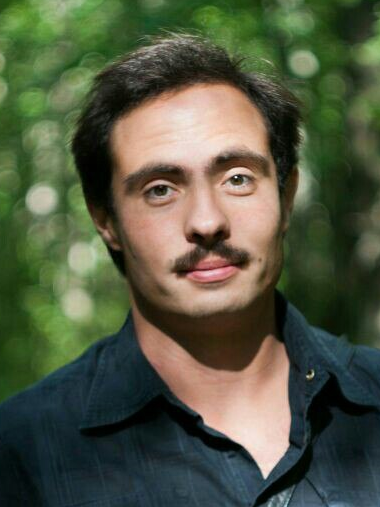
\includegraphics[width=1in,height=1.25in,clip,keepaspectratio]{Konyu10.png}}]{Ivan V. Konyukhov} was born in Kazan, Tatar Autonomous Soviet Socialist Republic, USSR, in 1989. He received his candidate degree in physics and mathematics from Kazan Federal University, Russian Federation in 2012. From 2012 till 2017, he had been working as a teaching assistant at the Applied Mathematics Department of Kazan Federal University. Since 2017, he has been a research fellow, postdoctoral researcher, assistant professor and associate professor at Innopolis University, Russian Federation. Nowadays he is also a head of High-Performance Computing Lab. He has authored six teaching aids, over 60 articles and 4 patents. His research interests include computational fluid dynamics, numerical simulations, digital twins, parallel and distributed programming, as well as applied artificial intelligence. 

He is also a program committee member of the International Conference on Computational Optimization (ICOMP).
\end{IEEEbiography}

\begin{IEEEbiography}[{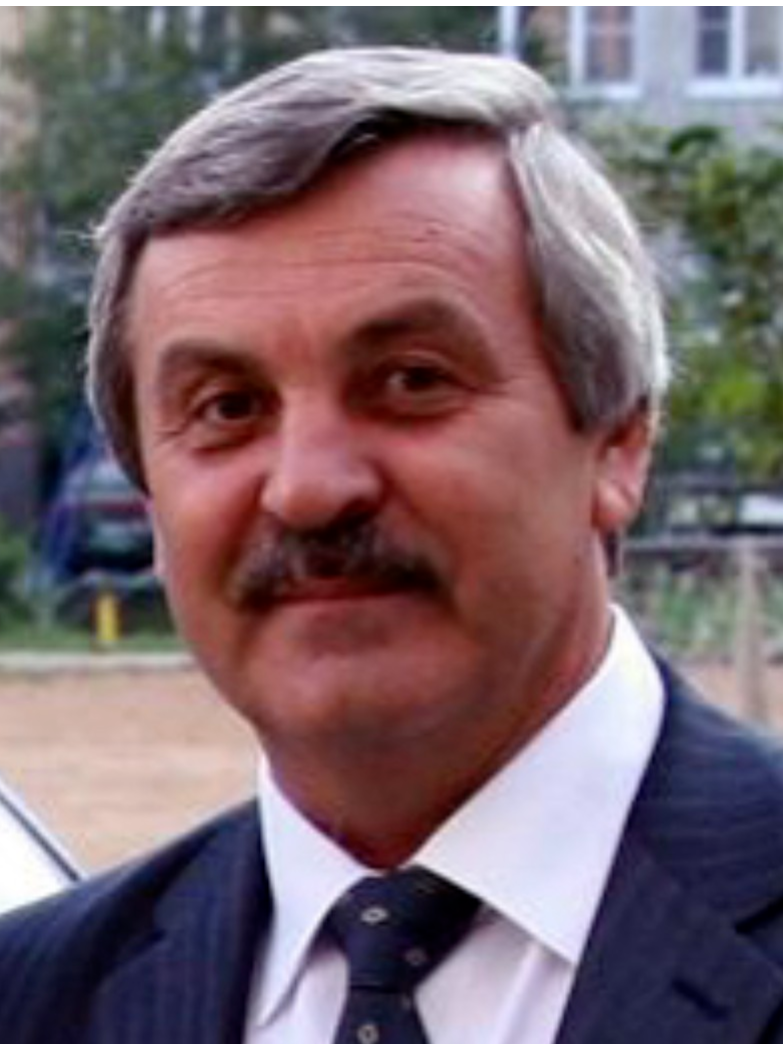
\includegraphics[width=1in,height=1.25in,clip,keepaspectratio]{Konyu11.png}}]{Vladimir M. Konyukhov} was born in Batumi, Georgia Soviet Socialist Republic, USSR, in 1956. He received his candidate and doctoral degrees in physics and mathematics from Kazan State University, USSR in 1988 and 2005, respectively. From 1984, he was a leading research fellow at the Chebotarev Institute of Mechanics and Mathematics and an associate professor at the Department of Applied Mathematics at the Institute of Computational Mathematics and Information Technologies. Since 2006, he has been a full professor at the department of applied mathematics and artificial intelligence at Kazan Federal University. He has authored five books, over 150 articles and more than 10 patents. His research interests include mathematical modeling of multi-phase flow in porous media and oil wells, simulation of pollutant migration in aquifers, numerical analysis of mass transfer in circulatory systems, numerical methods and computer visualization for physical processes, scientific machine learning and applied artificial intelligence. 

He is an associate editor of the proceedings of the International Conference on Parallel Computational Technologies and a member of the dissertation council at Kazan Federal University in the specialty "Mathematical Modeling, Numerical Methods and Software Packages" in the field of Physical and Mathematical Sciences.
\end{IEEEbiography}
\EOD

\end{document}


